\documentclass[../../main.tex]{subfiles}

\begin{document}

\chapter{Probability Distributions}

Most of the statistics and probabilities that we have worked with up until this point are used to summarise and analyse pre-existing data. However, it is often in our interest to use statistics to make predictions.

\section{Discrete Random Variables}
A \textbf{random variable} is a variable that mainly depends on chance. In a similar fashion to discrete and continuous data, random variables can be discrete or continuous. Discrete random variables take fixed values and each possible value has a certain probability of happening.

Notation for random variables is crucial. We use a capital letter to denote the variable itself and a lowercase letter to denote a specific instance of the variable. For example, if we had a random variable to demonstrate the outcome of a fair six-sided die, we could represent that by $X$. Then, if we were to roll a 4, we could say $x = 4$ for that roll.

Discrete random variables are often displayed in a table showing each possible value and its respective probability; this is known as the \textbf{probability distribution} of the variable.
\begin{example}{Discrete Random Variables}
A biased six-sided die has the faces 1, 2, 2, 3, 4, 4. Draw a table to show the distribution of this random variable.
\sep
We consider the possible outcomes of the die and the probability of each outcome occurring. The probability of rolling a 1 is $\frac{1}{6}$, rolling a 2 $\frac{2}{6}$ = $\frac{1}{3}$, a 3 $\frac{1}{6}$, and a 4 $\frac{1}{3}$.  We can construct a table as follows:
\begin{align}
\begin{tabular}{ |c|c|c|c|c| } 
 \hline
 $x$ & 1 & 2 & 3 & 4 \\ 
 \hline
 $P(X=x)$ & $\frac{1}{6}$ & $\frac{1}{3}$ & $\frac{1}{6}$ & $\frac{1}{3}$ \\ 
 \hline
\end{tabular}
\end{align}
\end{example}

A probability distribution may also be presented in an algebraic format, as shown in the following example.
\begin{example}{More Discrete Random Variables}
The discrete random variable $K$ is defined by the following:
\begin{align}
P(K=k) = \frac{1}{18}(4+k) \text{ for } k \in \{1, 2, 3\}
\end{align}
Draw a table to show the distribution of this random variable.
\sep
We are given a general expression for the probability; to obtain each specific value, we simply substitute 1, 2, or 3 for $k$. When $k = 1$, 
\begin{align}
P(K=1) &= \frac{1}{18}(4+1) \\ 
&=\frac{5}{18}
\end{align}
Repeating this for $k = 2$ and $k = 3$ results in the following:
\begin{align}
\begin{tabular}{ |c|c|c|c| } 
 \hline
 $x$ & 1 & 2 & 3 \\ 
 \hline
 $P(X=x)$ & $\frac{5}{18}$ & $\frac{1}{3}$ & $\frac{7}{18}$ \\ 
 \hline
\end{tabular}
\end{align}
\subtitle{Insight}
What do the probabilities add up to? Why must this be the case?
\end{example}

The \textbf{mode} of a random variable is the value that occurs the most frequently, i.e. has the highest probability. In Example 19.1.2, the mode would be 3 since it has the highest probability of occurring. The die in Example 19.1.1 can be described as \textbf{bimodal} because there are two values (2 and 4) that occur the most often.

\subsection{Expectation}
When we deal with random variables, we often ask ourselves what the ``average" value of the variable is. In statistics, we call this the \textbf{expectation} or \textbf{expected value} of the variable. The expectation of a discrete random variable $X$ is expressed as $E(X)$ and is given by:

{\hfill\Large\bfseries NEEDS FIXING\hfill}
\begin{lstlisting}
\begin{formula}
E(X) = \sum x \cdot P(X=x)
\end{formula}
 \end{lstlisting}

It is important to note that $E(X)$ does not have to be an actual value that you can obtain from one trial. It is instead what you would expect to get, on average, if you were to generate a value for the variable infinitely many times.

\begin{example}{Expectation of a Die}
What is the expected value of a fair six-sided die?
\sep
First, we can construct a table for the distribution.
\begin{align}
\begin{tabular}{ |c|c|c|c|c|c|c| } 
 \hline
 $x$ & 1 & 2 & 3 & 4 & 5 & 6 \\ 
 \hline
 $P(X=x)$ & $\frac{1}{6}$ & $\frac{1}{6}$ & $\frac{1}{6}$ & $\frac{1}{6}$ & $\frac{1}{6}$ & $\frac{1}{6}$ \\ 
 \hline
\end{tabular}
\end{align}
Drawing this table helps us to visualise expectation more easily. We can multiply the two numbers in each column and add up those products. This results in:
\begin{align}
E(X) &= 1 \cdot \frac{1}6 + 2 \cdot \frac{1}6 + 3 \cdot \frac{1}6 + 4 \cdot \frac{1}6 + 5 \cdot \frac{1}6 + 6 \cdot \frac{1}6 \\
&= \frac{7}2 \text{ or } 3.5
\end{align}
\end{example}

\begin{thinking}
How does the formula for expectation of a discrete random variable relate to the formula for the mean of a data set? Can we say that the mean and the expected value are the same thing?
\end{thinking}

\section{The Binomial Distribution}
Suppose you knew that in your area there is a 15\% chance that it will rain on any given day. How would you use this information to calculate the probability that it will rain on at least two days over the next week? Your intuition probably tells you to make a tree diagram, but that would be tedious and get hard to read very quickly! Could you use this information to calculate how many rainy days you would expect over the course of a week, a month, or even a year? Fortunately, we have a method of accomplishing this using a special type of probability distribution known as the \textbf{binomial distribution}. 

A binomial distribution can be used when dealing with an event that is repeated many times and each trial has a probability of ``success" and a probability of ``failure" (both of which must add up to 1). The trials must also be independent of each other.
\begin{theorem}{The Binomial Distribution}
The notation that we use for a binomial distribution is:
\begin{align}
    X \sim B(n, p)
\end{align}
where $n$ is the number of trials and $p$ is the probability of success for any given trial. We can also say that the probability that $x$ trials are successful is:
\begin{align}
    P(X=x) = \binom{n}{x}p^x(1-p)^{n-x}
\end{align}
\end{theorem}

The probability equation for the binomial distribution may look familiar; it is identical to the general term of the binomial expansion (the name somewhat gives it away!). You may wonder how this is true, but we can explore this with a simple example.

Consider a game where a fair six-sided die is rolled 3 times in succession and the game is won if exactly one roll is a 6. Although a die technically has six possible outcomes, in this scenario there are only 2 that we are concerned with: ``a 6" or ``not a 6." We may ask ourselves at this point: ``What is the probability of winning this game?" Winning this game requires a 6 to be rolled once \textit{and} a ``non-6" to be rolled twice. The probability of rolling a 6 is $\frac{1}6$ and the probability of not rolling a 6 is $\frac{5}6$. This suggests that the probability of winning is equal to:
\begin{align}
    \bigg(\frac{1}6\bigg) \cdot \bigg(\frac{5}6\bigg)^2
\end{align}
However, we are not done. The rules of the game do not dictate that the 6 must be rolled first, second, or third. Therefore, we must multiply our probability by 3. So, our final probability is:
\begin{align}
    3 \cdot \bigg(\frac{1}6\bigg) \cdot \bigg(\frac{5}6\bigg)^2
\end{align}
which can be rewritten as:
\begin{align}
    \binom{3}{1} \cdot  \bigg(\frac{1}6\bigg)^1 \cdot \bigg(\frac{5}6\bigg)^2
\end{align}
This should ring a bell to you; it looks identical to the binomial theorem. Let's work through some examples.
\begin{example}{Rainy Days}
The chance of rain in a certain town on any given day is 0.15. \\
(a) What is the probability that it rains on exactly 2 days over a week? \\
(b) What is the probability that it rains on at least 2 days over a week?
\sep
There is a 15\% chance of rain on one day and there are 7 days in a week. We can therefore write the distribution as: $X \sim B(7, \, 0.15)$. \\
(a) We can simply apply our probability formula for $x = 2$.
\begin{align}
    P(X=2) &= \binom{7}{2}(0.15)^2(0.85)^5 \\
    &= 0.210 \text{ (3sf)}
\end{align}
(b) This is slightly less straightforward as we have no way of calculating $P(X \geq 2)$ by hand. We could calculate $P(X=2) + P(X=3) + \cdots + P(X=7)$ but this is time-consuming; we could instead consider the complement. The complement of $P(X \geq 2)$ is $P(X < 2)$, or $P(X=0) + P(X=1)$, and our answer will be 1 minus that.
\begin{align}
    P(X \geq 2) &= 1 - (P(X=0) + P(X=1)) \\
    &= 1 - P(X=0) - P(X=1) \\
    &= 1 - \binom{7}{0}(0.15)^0(0.85)^7 - \binom{7}{1}(0.15)^1(0.85)^6 \\
    &= 0.283 \text{ (3sf)}
\end{align}
\end{example}

Your calculator can quickly calculate binomial probabilities. It also has a special function to instantly calculate a range of probabilities as in part (b) above; this is known as a \textbf{cumulative probability}.

Calculating the expectation of a binomial distribution is not necessarily the same as for a normal discrete random variable. From our rainy day example from above, we know that the chance of rain on \textit{one} day is 0.15. No matter whether or not it rains today, we know that the probability that it will rain tomorrow is also 0.15. As we add more days, the pattern continues: we keep adding 0.15 for every day, which suggests a general formula for the expected value of the binomial distribution:

{\hfill\Large\bfseries NEEDS FIXING\hfill}
\begin{lstlisting}
\begin{formula}
X \sim B(n, p) \implies E(X) = np
\end{formula}
 \end{lstlisting}

There is also a formula to calculate the \textbf{variance} or spread of the distribution, which is as follows:

{\hfill\Large\bfseries NEEDS FIXING\hfill}
\begin{lstlisting}
\begin{formula}
X \sim B(n, p) \implies Var(X) = np(1-p)
\end{formula}
 \end{lstlisting}

This can be proved algebraically but it is beyond the scope of our course - you can explore it yourself.
\begin{example}{Guessing on a Test}
A multiple-choice test contains 20 questions with four possible answers each, one of which is correct. If one were to blindly guess the answer to each question, how many correct answers would they expect?
\sep
Although it's advised to never follow this brutal guessing approach in a test, we can calculate the expected number of correct answers as follows:
\begin{align}
    X &\sim B(20, \, 0.25) \\
    E(X) &= 20 \cdot 0.25 \\
    &= 5
\end{align}
\end{example}

You should be able to recognise that a question is talking about a binomial distribution; most exam questions will not explicitly tell you to use a certain distribution. Look out for an event that occurs multiple times and has two possible outcomes.

\newpage

\section{Theory of Continuous Random Variables (HL Only)}
As we saw in the previous two sections, random variables can be discrete or continuous. We are yet to consider the case of a continuous random variable (CRV), which are variables where taking an exact value would not only be impractical but also virtually impossible.

For example, suppose we were observing birds that are known to have a wingspan of 25 cm. Our measuring instrument may tell us that one specific bird's wingspan is 25.0 cm, but due to the uncertainty in the reading we cannot say for sure that the wingspan is \textit{exactly} 25.0 cm. For all we know, it could be 25.0042069\dots cm, and even then the most precise apparatus possible would still be unable to tell us the exact value. 

Therefore, with CRVs, we cannot refer to the probability of the variable taking an exact value (that would in fact be treated as zero - you may want to think about why this is). Instead, we have to refer to the probability of the variable falling within a range.

With an infinite number of possible values for a CRV, how could we represent the distribution in a more comprehensible way? What is done in practice is graphing the probabilities as a function. If you were to choose two points on the curve, you could find the probability of the variable being in between those two points by taking the area under the curve between those two points. To understand why this is, recall that the probability of a CRV taking an exact value is treated as zero. Similarly, a definite integral with the same lower and upper bound will evaluate to zero.

Since probability corresponds to area, it makes sense to assume that our probability function must have a total area underneath it of 1. This is in fact a defining property of a \textbf{probability density function}, which is the name we give for a function that shows the probability distribution of a CRV.

\begin{theorem}{The Probability Density Function}
For any continuous random variable $X$ with probability density function $f(x)$, the probability of the variable lying between any two values $a$ and $b$ ($b > a$) is:
\begin{align}
    P(a<x<b) = \int_a^b f(x) \mathrm dx
\end{align}
For all probability density functions, it must hold that
\begin{align}
    \int_{-\infty}^{\infty} f(x) \mathrm dx = 1
\end{align}
\end{theorem}

You may notice that we set the bounds of integration to positive and negative infinity. This is because a CRV \textit{can} hypothetically take any value (so long as it is a real number) but that is hardly ever the case in practice. The bounds will just be set to whatever the lowest and highest possible values of the variable can be. Using these definitions, we can start to solve problems involving CRVs.
\begin{example}{Manipulating Variables}
The continuous random variable $X$ has the following probability density function:
$$f(x) = 
        \begin{cases}
            kx^2 & \quad 0 < x < 3 \\
            0 & \quad \text{otherwise}
        \end{cases}
$$
What is the value of $k$? 
\sep
We know that the area under the curve must equal 1 and we know the function, so we can set up an integral as follows:
\begin{align}
    \int_0^3 kx^2 \mathrm dx = 1
\end{align}
Evaluating the integral on the LHS using the power rule gives us:
\begin{align}
    {\Big[\frac{k}3 x^3\Big]}_0^3 &= 1 \\
    9k + 0 &= 1 \\
    k &= \frac{1}9
\end{align}
\end{example}

Just like with discrete random variables, we can find certain properties of CRVs.

{\hfill\Large\bfseries NEEDS FIXING\hfill}
\begin{lstlisting}
\begin{formula}
E(X) = \int_{-\infty}^{\infty} xf(x) \mathrm dx $$$$
E(X^2) = \int_{-\infty}^{\infty} x^2f(x) \mathrm dx $$$$
Var(X) = E(X^2) - [E(X)]^2
\end{formula}
 \end{lstlisting}

As for the median, by definition, half of the data should lie below it and half above it. This means that we want a point $m$ such that the area under the curve from the minimum value to that point equals one half.

{\hfill\Large\bfseries NEEDS FIXING\hfill}
\begin{lstlisting}
\begin{formula}
\int_{-\infty}^m f(x) \mathrm dx = \frac{1}2 \\
\end{formula}
 \end{lstlisting}
The mode will be where the function has its maximum value. Be warned that this does \textit{not} always mean setting the first derivative of the function equal to zero. You will have to graph the function to see whether it is increasing, decreasing, or a bit of both.
\begin{example}{Getting our Hands Dirty}
Consider the following probability density function:
$$f(x) = 
        \begin{cases}
            x - \frac{1}{4}x^3 & \quad 0 < x < 2 \\
            0 & \quad \text{otherwise}
        \end{cases}
$$
Find the mean, median and mode of the random variable associated with this function. 
\sep
For the mean/expected value, you could just evaluate the definite integral on your calculator, but make sure to practice setting up and manipulating the integral as that will get you crucial method marks on your exam.
\begin{align}
    E(X) &= \int_0^2 x(x - \frac{1}{4}x^3) \mathrm dx \\
    &= \int_0^2 x^2- \frac{1}{4}x^4 \mathrm dx \\
    &= 1.07 \text{ (3sf)}
\end{align}
Next, let's find the median. We need an $m$ that will make the integral equal to $\frac{1}2$.
\begin{align}
    \int_0^m x - \frac{1}{4}x^3 \mathrm dx &= \frac{1}2 \\
    \Big[\frac{1}{2}x^2 - \frac{1}{16}x^4\Big]_0^m &= \frac{1}2 \\
    \frac{1}{2}m^2 - \frac{1}{16}m^4 &= \frac{1}2
\end{align}
This is a disguised quadratic which can be solved by substituting a new variable (we'll use $k$) for $m^2$.
\begin{align}
    \frac{1}{2}k - \frac{1}{16}k^2 - \frac{1}2 &= 0 \\
    \frac{1}{16}k^2 - \frac{1}{2}k + \frac{1}2 &= 0
\end{align}
To clean up the fractions, we can multiply everything by 16.
\begin{align}
   k^2 - 8k + 8 &= 0
\end{align}
Using the quadratic formula,
\begin{align}
    k &= \frac{-(-8) \pm \sqrt{(-8)^2 - 4\cdot1\cdot8}}{2 \cdot 1} \\
    &= \frac{8 \pm \sqrt{32}}{2} \\
    &= 4 \pm \sqrt{8} \textit{ (Don't round yet!)}
\end{align}
Since $k = m^2$, let's find the values of $m$.
\begin{align}
    m &= \sqrt{4 - \sqrt{8}} \text{ or } \sqrt{4 + \sqrt{8}} \\
    &= 1.08 \text{ or } 2.61 \text{ (3sf)}
\end{align}
The second value of $m$ is outside the domain of the function, so we disregard it. Therefore, the median is 1.08.

Now for the mode, we will first have to graph the function and interpret the maximum value.
\begin{center}
    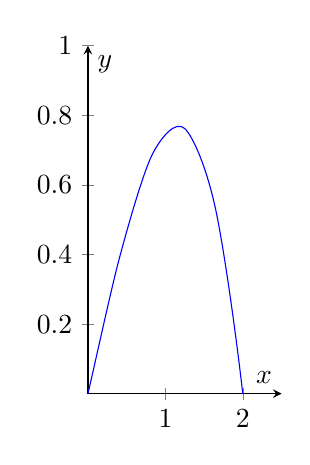
\begin{tikzpicture}
        \begin{axis}
        [height=6cm,width=\textwidth/3,
        axis y line = center,
        axis x line = middle,
        xlabel=$x$,ylabel=$y$,
        xmin=0,xmax=2.5, ymin=0,ymax=1]
            \addplot[smooth, blue, mark = none]{x - (x^3)/4};
        \end{axis}
    \end{tikzpicture}
\end{center}
We can clearly see that the maximum value occurs at a stationary point, so it will satisfy $f'(x) = 0$. Your calculator can tell you this value right away, but you should get into the habit of working it out algebraically. Differentiating our function using the power rule gives us:
\begin{align}
    \frac{\mathrm d}{\mathrm dx}\Big(x - \frac{1}{4}x^3\Big) = 1 - \frac{3}{4}x^2
\end{align}
Setting our first derivative equal to zero and solving for $x$ gives us:
\begin{align}
    1 - \frac{3}{4}x^2 &= 0 \\
    \frac{3}{4}x^2 &= 1 \\
    x^2 &= \frac{4}{3} \\
    \implies x &= \frac{2}{\sqrt{3}} = 1.15 \text{ (3sf)}
\end{align}
Note that we take the positive square root to stay within the domain of our function.
\end{example}

\newpage

\section{The Normal Distribution}

Most of the probability density functions that we encountered in the previous sections were purely theoretical examples. In real-life examples, however, the value of a CRV is much more likely to be near its average value. One distribution that is very commonly used in such a scenario is known as the \textbf{normal distribution}. 

The normal distribution has an instantly recognisable bell-shaped curve
\pgfmathdeclarefunction{gauss}{2}{
  \pgfmathparse{1/(#2*sqrt(2*pi))*exp(-((x-#1)^2)/(2*#2^2))}
}
\begin{center}
    \begin{tikzpicture}
        \begin{axis}
        [height=6cm,width=\textwidth/2,
        axis y line = center,
        axis x line = middle,
        xlabel=$x$,ylabel=$y$,
        xmin=-3,xmax=3, ymin=0,ymax=1]
            \addplot[smooth, blue, mark = none]{gauss(0,1)};
        \end{axis}
    \end{tikzpicture}
\end{center}
\section{The Inverse Normal Distribution}

\end{document}